\documentclass{standalone}
\usepackage{../../../../preamble_formulas}

\begin{document}
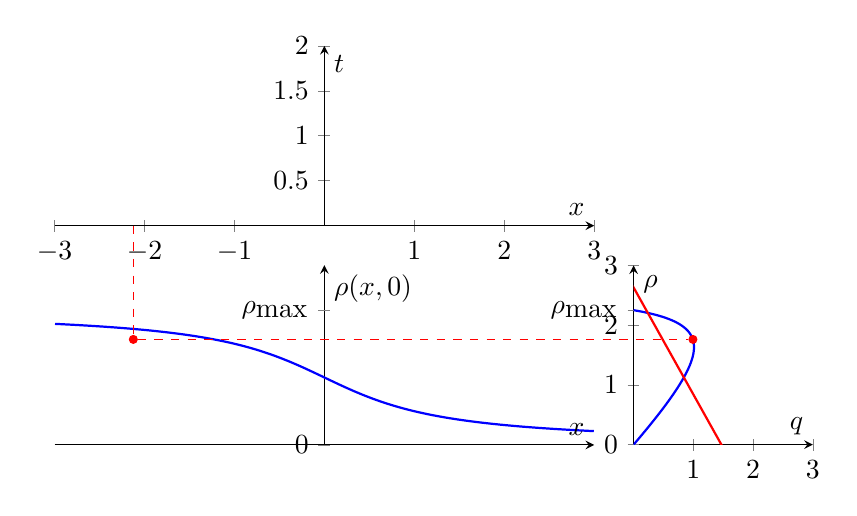
\begin{tikzpicture}
  \def\X{3}
  \def\Y{2}
  \def\eps{0.072}
  \begin{axis}[
      name=plot1,
      axis lines=middle,
      xmin=-\X, xmax=\X,
      ymin=0, ymax=\Y,
      %xtick=\empty, ytick=\empty,
      ylabel={$t$},
      xlabel={$x$},
      axis equal image,
      %axis on top,
    ]
    % \def\xmax{\pgfkeysvalueof{/pgfplots/xmax}}
    % \def\xmin{\pgfkeysvalueof{/pgfplots/xmin}}
    % \def\ymax{\pgfkeysvalueof{/pgfplots/ymax}}
    % \def\ymin{\pgfkeysvalueof{/pgfplots/ymin}}
    % \addplot [thick,samples=400,smooth,blue,domain=\xmin:0]
    % ({-x^2}, {x});
    % \addplot[thick,samples=400,smooth,red,domain=0:\xmax] ({-x^2}, {x});
  \end{axis}

  \begin{axis}[
      name=plot2,
      at=(plot1.south),
      anchor=north,
      yshift=-0.5cm,
      axis lines=middle,
      xmin=-\X, xmax=\X,
      ymin=0, ymax=\Y,
      xtick=\empty, ytick=\empty,
      extra y ticks = {0,1.5},
      extra y tick labels={0,$\rho_{\textrm{max}}$},
      ylabel={$\rho(x,0)$},
      xlabel={$x$},
      axis equal image,
      restrict x to domain=-\X:\X,
      %axis on top,
    ]
    \addplot[thick,samples=400,smooth,blue]{3/2*(rad(atan(-x))/pi+0.5)};
  \end{axis}
  \begin{axis}[scale=0.4,
      name=plot3,
      at=(plot2.east),
      anchor=west,
      xshift=0.5cm,
      axis lines=middle,
      xmin=0, xmax=\X,
      ymin=0, ymax=\X,
      %xtick=\empty, ytick=\empty,
      extra y ticks = {0,2.25},
      extra y tick labels={0,$\rho_{\textrm{max}}$},
      ylabel={$\rho$},
      xlabel={$q$},
      axis equal image,
      % y=2cm/\Y,
      % x=2cm/2/\X,
      %axis on top,
    ]
    \addplot[thick,samples=400,smooth,blue,domain=0:2.25]({-(-x+0.3802+2.25)-1/(-x+0.3802+2.25)+3.0104},{x});
    \addplot[thick,samples=10,smooth,red]{1.125-1.790122*(x-0.8408364)};
  \end{axis}
  \node (11) at ({-2+\X},{-1-\eps-(1.5-1.127862457)})  [shape=circle,draw=red,inner sep=0pt,minimum size=0.1cm,fill=red] {};
  \node (12) at ({2*\X+0.5+\eps+1.535},{-1-\eps-(1.5-1.127862457)})  [shape=circle,draw=red,inner sep=0pt,minimum size=0.1cm,fill=red] {};

  \draw[red,dashed] ({-2+\X},0) -- (11) -- (12);
\end{tikzpicture}

\end{document}